
% ibs.tex

\documentclass[10pt,a4paper,titlepage]{article}
\usepackage[czech]{babel}
\usepackage[utf8]{inputenc}
\usepackage[margin=100pt]{geometry}
    
\usepackage{graphicx}   % Import pictures
\usepackage{multicol}
\usepackage{caption}
\usepackage{subcaption}
%\usepackage{csquotes}

\usepackage[backend=biber, sorting=none]{biblatex}
\addbibresource{ibs.bib}
    
\begin{document}
  \pagenumbering{gobble}

  \begin{center}
    \section*{Analýza aplikačního protokolu zabezpečeného SSL/TLS}
    Martin Beneš
  \end{center}

  \section*{Úvod}
  SSL/TLS jsou protokoly, řešící důvěrnost komunikace typu klient-server pomocí šifrování.
  Zajišťují také autentizaci, integritu a nepopiratelnost. Pracují mezi aplikační a
  transportní vrstvou, vyžadují spolehlivý přenost, tedy většinou na TCP, umožňují šifrovat
  komunikaci existujících aplikačních protokolů (email - SMTP, www - HTTP).
  Vyžadují autentizaci serveru (pomocí certifikátu) klientem, nepovinně také vice versa
  klienta serveru. \cite{DigiCert} \cite{RootSsl}

  \begin{figure}[h!]
    \begin{center}
      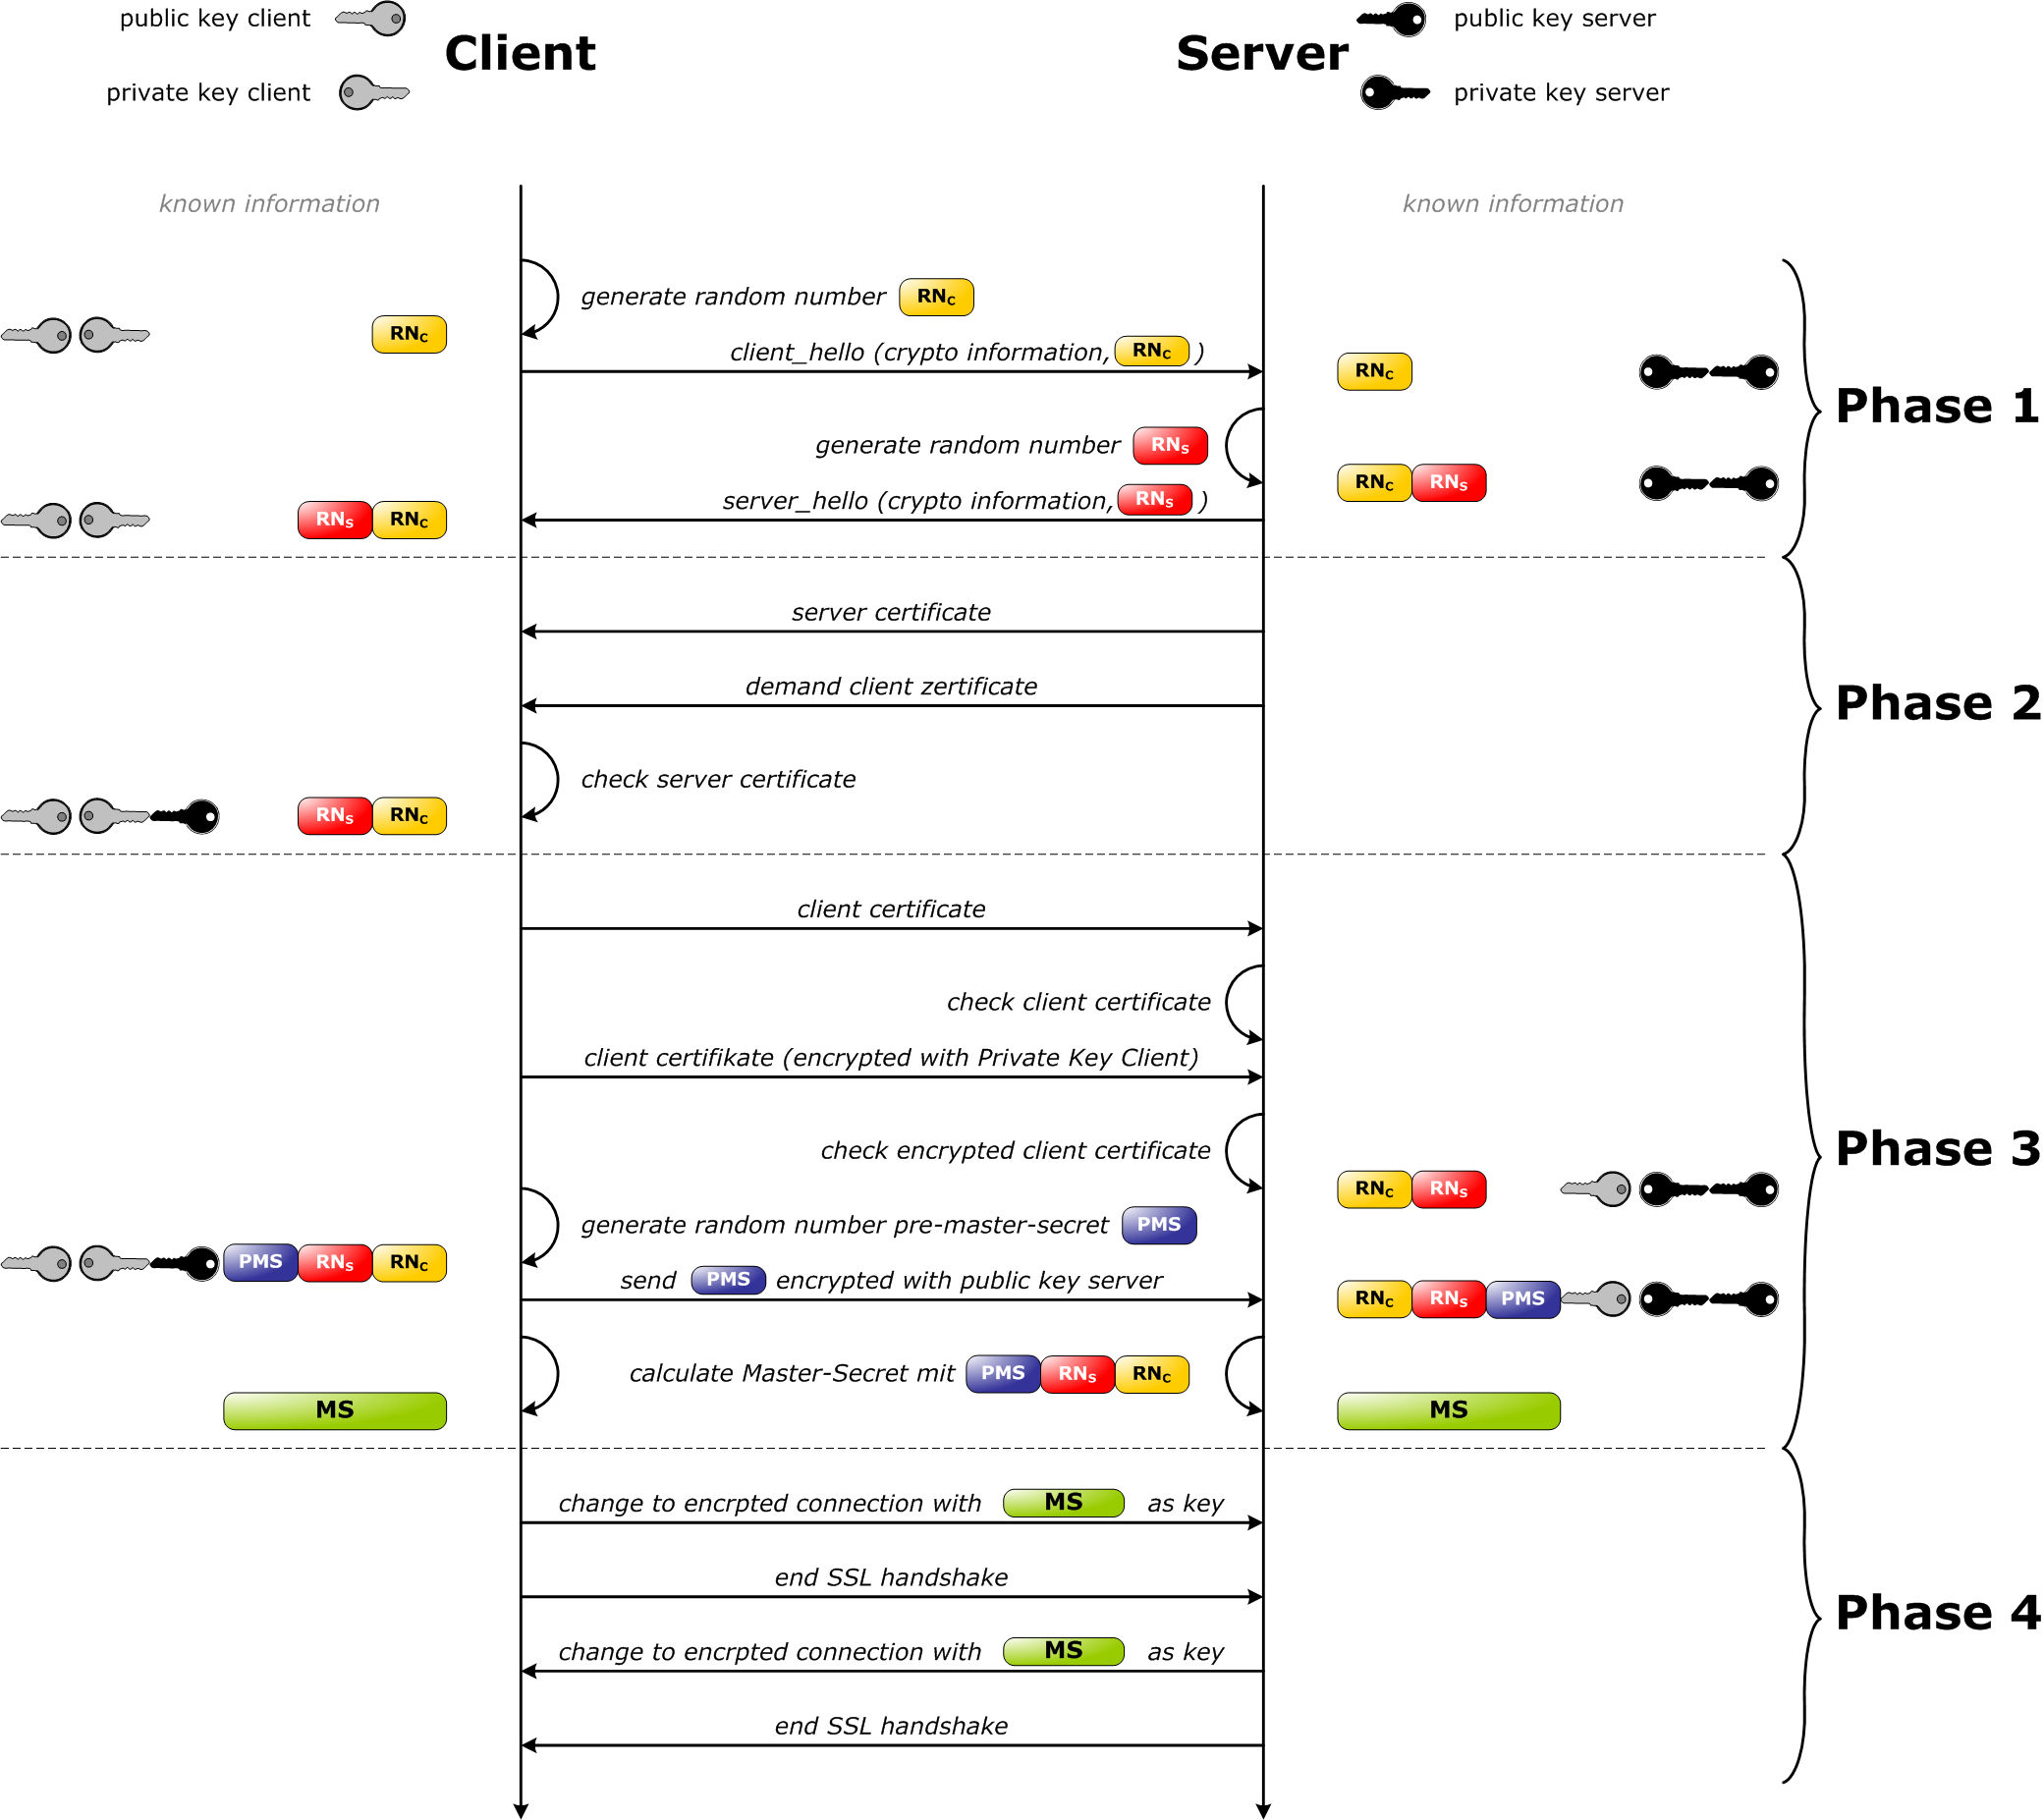
\includegraphics[width=0.6\textwidth]{ssl.png}
      \caption{Schéma SSL handshake\label{fig:sslhandshake} \cite{WikiSSL}}
    \end{center}    
  \end{figure}

  TLS navazuje na SSL protokol, po SSL 3.0 z roku 1996 vyšel v roce 1999 TLS 1.0.
  Fakticky jsou si velmi podobné, SSL 3.0 (dokonce i TLS 1.0) je dnes považován obecně
  za nezabezpečený, je možné jej prolomit BEAST útokem. Novější verze TLS se snaží
  odstraňovat chyby a zamezovat útokem, a jsou považovány za marginálně bezpečnější.
  \cite{LuxSci}

  \subsection*{Zranitelnosti}
  Na SSL/TLS protokoly je popsáno několik možností útoků. Dvěma nejznámějšími
  jsou SSL Beast a SSL/TLS renegotiation.
  
  \paragraph{SSL Beast}
  SSL Beast je útok na straně klienta, založen na dešifrování tajné zprávy.
  Funguje na SSL a TLS 1.0, zabezpečenými blokovou šifrou (AES, DES), na proudové
  šifry je neúčinný. \cite{sslbeast}

  \paragraph{SSL/TLS renegotiation}
  SSL/TLS renegotiation (znovuvyjednání) je útok nad SSL/TLS na principu MITM.
  Uplatňuje se v průběhu SSL/TLS handshake fáze. Je funkční na SSL 3.0 a TLS.
  Útočník naruší obsah zprávy, je schopen zasílat příkazy serveru (např. HTTP),
  který je zpracovává jako od legitimního klienta. \cite{sslrenegotiation}

  
  \section*{Realizace útoku}

  \section*{Zhodnocení výsledků}


  
  
  % references
  \printbibliography

\end{document}